\documentclass[a4paper,11pt]{article}
\usepackage{amsmath,amsthm,amsfonts,amssymb,amscd,amstext,vmargin,graphics,graphicx,tabularx,multicol} 
\usepackage[francais]{babel}
\usepackage[utf8]{inputenc}  
\usepackage[T1]{fontenc} 
\usepackage{pstricks-add,tikz,tkz-tab,variations}
\usepackage[autolanguage,np]{numprint} 
\usepackage{calc}
\usepackage{mathrsfs}

\setmarginsrb{1.5cm}{0.5cm}{1cm}{0.5cm}{0cm}{0cm}{0cm}{0cm} %Gauche, haut, droite, haut
\newcounter{numexo}
\newcommand{\exo}[1]{\stepcounter{numexo}\noindent{\bf Exercice~\thenumexo} : }
\reversemarginpar

\newcommand{\bmul}[1]{\begin{multicols}{#1}}
\newcommand{\emul}{\end{multicols}}

\newcounter{enumtabi}
\newcounter{enumtaba}
\newcommand{\q}{\stepcounter{enumtabi} \theenumtabi.  }
\newcommand{\qa}{\stepcounter{enumtaba} (\alph{enumtaba}) }
\newcommand{\initq}{\setcounter{enumtabi}{0}}
\newcommand{\initqa}{\setcounter{enumtaba}{0}}

\newcommand{\be}{\begin{enumerate}}
\newcommand{\ee}{\end{enumerate}}
\newcommand{\bi}{\begin{itemize}}
\newcommand{\ei}{\end{itemize}}
\newcommand{\bp}{\begin{pspicture*}}
\newcommand{\ep}{\end{pspicture*}}
\newcommand{\bt}{\begin{tabular}}
\newcommand{\et}{\end{tabular}}
\renewcommand{\tabularxcolumn}[1]{>{\centering}m{#1}} %(colonne m{} centrée, au lieu de p par défault) 
\newcommand{\tnl}{\tabularnewline}

\newcommand{\trait}{\noindent \rule{\linewidth}{0.2mm}}
\newcommand{\hs}[1]{\hspace{#1}}
\newcommand{\vs}[1]{\vspace{#1}}

\newcommand{\N}{\mathbb{N}}
\newcommand{\Z}{\mathbb{Z}}
\newcommand{\R}{\mathbb{R}}
\newcommand{\C}{\mathbb{C}}
\newcommand{\Dcal}{\mathcal{D}}
\newcommand{\Ccal}{\mathcal{C}}
\newcommand{\mc}{\mathcal}

\newcommand{\vect}[1]{\overrightarrow{#1}}
\newcommand{\ds}{\displaystyle}
\newcommand{\eq}{\quad \Leftrightarrow \quad}
\newcommand{\vecti}{\vec{\imath}}
\newcommand{\vectj}{\vec{\jmath}}
\newcommand{\Oij}{(O;\vec{\imath}, \vec{\jmath})}
\newcommand{\OIJ}{(O;I,J)}


\newcommand{\reponse}[1][1]{%
\multido{}{#1}{\makebox[\linewidth]{\rule[0pt]{0pt}{20pt}\dotfill}
}}

\newcommand{\titre}[5] 
% #1: titre #2: haut gauche #3: bas gauche #4: haut droite #5: bas droite
{
\noindent #2 \hfill #4 \\
#3 \hfill #5

\vspace{-1.6cm}

\begin{center}\rule{6cm}{0.5mm}\end{center}
\vspace{0.2cm}
\begin{center}{\large{\textbf{#1}}}\end{center}
\begin{center}\rule{6cm}{0.5mm}\end{center}
}



\begin{document}
\pagestyle{empty}
\titre{Séance d'exercices: Résolution d'équation du premier degré}{}{}{3ème}{}

\vspace*{0.2cm}


{\large \textbf{\underline{PARTIE A :}}  Résolution d'équation}\\

\vspace*{0.2cm}

\exo \\


\initq \textbf{\qa} On considère l'équation suivante : \hspace*{0.5cm} $ 5x + 3(8-2x) = 15-(x-9)$\\
\textbf{4 est-il solution de l'équation ?}\\

\qa On considère l'équation suivante : \hspace*{0.5cm} $(3x+2)^{2} = 9x^{2} + 6x + 4$\\
\textbf{-2 est-il solution de l'équation ?}

\vspace{0.5cm}

\exo 

Résoudre les équations suivantes.


\bmul{3}
\initqa 

\qa $-2+x=11$\\


\qa $\dfrac{3}{4}x=5$


\columnbreak

\qa $9+x=44$\\

\qa $3x=27$


\columnbreak

\qa $-6 +x =-41$\\

\qa $-6x=-42$


\emul

\vspace*{0.5cm}

\exo 

Résoudre les équations suivantes.


\bmul{3}
\initqa 

\qa $ 4x - 3 = 79$ \\

\qa $4x-7 = 3x+8$




\columnbreak

\qa $6-8x=16x$\\


\qa $-x+11 = \dfrac{3}{5} x+3$




\columnbreak

\qa $50 = -2x + 35$\\

\qa $-2x +5 = -8x + 10$



\emul

\vspace*{0.2cm}

{\large \textbf{\underline{PARTIE B :}} Mise en équation} \\

\vspace*{0.25cm}


 
 
 
 \exo
 
 Trouve un nombre sachant que son triple augmenté de 2 est égal à son double augmenté de 3.

\vspace*{0.5cm}

 
 \exo

Thomas a obtenu 11 et 16 aux deux premiers contrôles de Maths.\\
Quelle note doit-il avoir au troisième contrôle pour obtenir 15 de moyenne ?



\vspace*{0.5cm}

 
 \exo
 Titeuf est passionné par son roman. Il a lu 260 pages en 3 jours. \\
 Le deuxième jour, il a lu deux fois plus de pages que le premier jour, et le troisième jour 20 pages de plus que le deuxième jour. \\
 Combien a-t-il lu de pages
le premier jour ?\\


  \bmul{2}
 \exo
 

Tous les cubes ont la même masse.\\
La balance est en équilibre.\\
Quelle est la masse d'une cube ?\\
On note m la masse d'un cube en kg.\\


\includegraphics[scale=0.8]{balanceexo.eps} 


\columnbreak

 
 \exo
 


x désigne un nombre supérieur à 1.
ABCD est un trapèze dont les côtés parallèles [AD] et [BC] ont des longueurs variables.\\
Existe-t-il un nombre x pour lequel ABCD est un
parallélogramme ?\\
Si oui, préciser la nature de ABCD.\\

\begin{center}
\includegraphics[scale=0.8]{exoequation.eps} 

\end{center}
\emul
\end{document}
